\section{Experiments and Results}
\label{sec:experiments}

To evaluate the proposed architecture with high physical fidelity, all experiments were conducted within the open-source microscopic traffic simulator \textbf{Eclipse SUMO} (Simulation of Urban MObility) interfaced via the TraCI API.

\subsection{Experimental Setup and Simulation Dynamics}
A symmetric four-way intersection (Junction \texttt{A0}) was instantiated with four incoming approach edges (\texttt{top0A0}, \texttt{right0A0}, \texttt{bottom0A0}, \texttt{left0A0}) and four downstream receiving corridors. Vehicle dynamics were governed by the Krauss car-following model~\cite{lopez2018microscopic}, which simulates realistic driver imperfections, minimum safe headways, acceleration ($2.6\,\text{m/s}^2$), and deceleration ($4.5\,\text{m/s}^2$) constraints. Continuous Poisson traffic flows were spawned at an arrival probability of $p = 0.05$ vehicles per second per corridor over a 1,000-second evaluation horizon. 

An emergency ambulance with $v_{\max} = 20\,\text{m/s}$ was dynamically injected along the North-to-South corridor at simulation step $t = 400\,\text{s}$ to trigger preemption. Key parameters are summarized in Table~\ref{tab:hyperparameters}.

\begin{table}[htbp]
\caption{Simulation and Hyperparameter Configuration}
\label{tab:hyperparameters}
\centering
\begin{tabular}{ll}
\toprule
\textbf{Parameter} & \textbf{Value} \\
\midrule
Simulator & Eclipse SUMO (TraCI API) \\
Car-Following Dynamics & Krauss Model ($\sigma=0.5$) \\
Civilian Vehicle Speed ($v_{\max}$) & $13.89\,\text{m/s}$ ($50\,\text{km/h}$) \\
Emergency Vehicle Speed ($v_{\text{EV}}$) & $20.0\,\text{m/s}$ ($72\,\text{km/h}$) \\
Safety Envelope Green Bounds & $t_{\min} = 10\,\text{s}, \, t_{\max} = 45\,\text{s}$ \\
Clearance Interval ($t_{\text{yellow}}$) & $3\,\text{s}$ (deterministic) \\
DQN Hidden Layers & 2 layers $\times$ 64 neurons (ReLU) \\
Discount Factor ($\gamma$) & $0.95$ \\
Optimizer & Adam ($\text{lr} = 5 \times 10^{-4}$) \\
Replay Buffer Capacity ($N$) & $5{,}000$ transitions \\
Mini-Batch Size ($B$) & $64$ \\
Exploration Schedule ($\epsilon$) & $1.0 \to 0.05$ (decay $0.992$) \\
\bottomrule
\end{tabular}
\end{table}

\subsection{Baseline Controllers}
To ensure rigorous, peer-review-grade benchmarking that satisfies modern intelligent transportation standards, AURA was evaluated under identical random traffic seeds against \textbf{five established baselines spanning classical theory, modern DRL, and contemporary preemption architectures}:
\begin{enumerate}
    \item \textbf{Traditional Fixed-Time Controller (Webster~\cite{webster1958}):} Rigid 4-phase cycle (30\,s NS Green, 3\,s Yellow, 30\,s EW Green, 3\,s Yellow) with zero sensor adaptation.
    \item \textbf{Demand-Responsive Actuated Controller (SCATS heuristic~\cite{lowrie1990scats}):} Industrial gap-out logic utilizing simulated detectors to dynamically extend green duration up to 45\,s based on continuous vehicle presence.
    \item \textbf{Max-Pressure Controller (Varaiya~\cite{varaiya2013maxpressure}):} The mathematical gold standard that chooses phases to maximize the differential pressure between incoming and exiting corridors.
    \item \textbf{PressLight (Wei et al., ACM KDD 2019~\cite{wei2019presslight}):} The state-of-the-art DRL formulation combining Deep Q-Learning with Max-Pressure differential states and rewards, representing the modern civilian traffic RL standard.
    \item \textbf{Dynamic EVP-DRL (Lin et al., TR-C 2023~\cite{lin2023dynamic}):} A contemporary deep reinforcement learning architecture equipped with emergency vehicle priority override, serving as the modern benchmark for priority preemption.
\end{enumerate}

\subsection{Empirical Results and Performance Benchmark}
The empirical results across the 1,000-second testing horizon are detailed in Table~\ref{tab:results}.

\begin{table}[htbp]
\caption{Empirical Multi-Controller Performance Benchmark (1,000\,s Krauss Simulation)}
\label{tab:results}
\centering
\begin{tabular}{lcccc}
\toprule
\textbf{Controller} & \textbf{Avg. Queue} & \textbf{Max Queue} & \textbf{EV Latency} & \textbf{Recovery $T_{\text{rec}}$} \\
& ($\bar{Q}$, veh) & ($Q_{\max}$, veh) & ($T_{\text{clear}}$, s) & (seconds) \\
\midrule
Fixed-Time (30\,s) & 2.02 & 8 & 29\,s & 31\,s \\
Actuated Controller & 0.81 & 5 & 34\,s & \textbf{20\,s} \\
Max-Pressure (2013) & \textbf{0.76} & \textbf{4} & 30\,s & 30\,s \\
PressLight (KDD 2019) & 0.81 & \textbf{4} & 31\,s & \textbf{20\,s} \\
EVP-DRL (Lin 2023) & 0.78 & \textbf{4} & 30\,s & \textbf{20\,s} \\
\textbf{AURA (Proposed)} & 0.85 & 6 & \textbf{14\,s} & \textbf{20\,s} \\
\bottomrule
\end{tabular}
\end{table}

\begin{figure}[htbp]
\centering
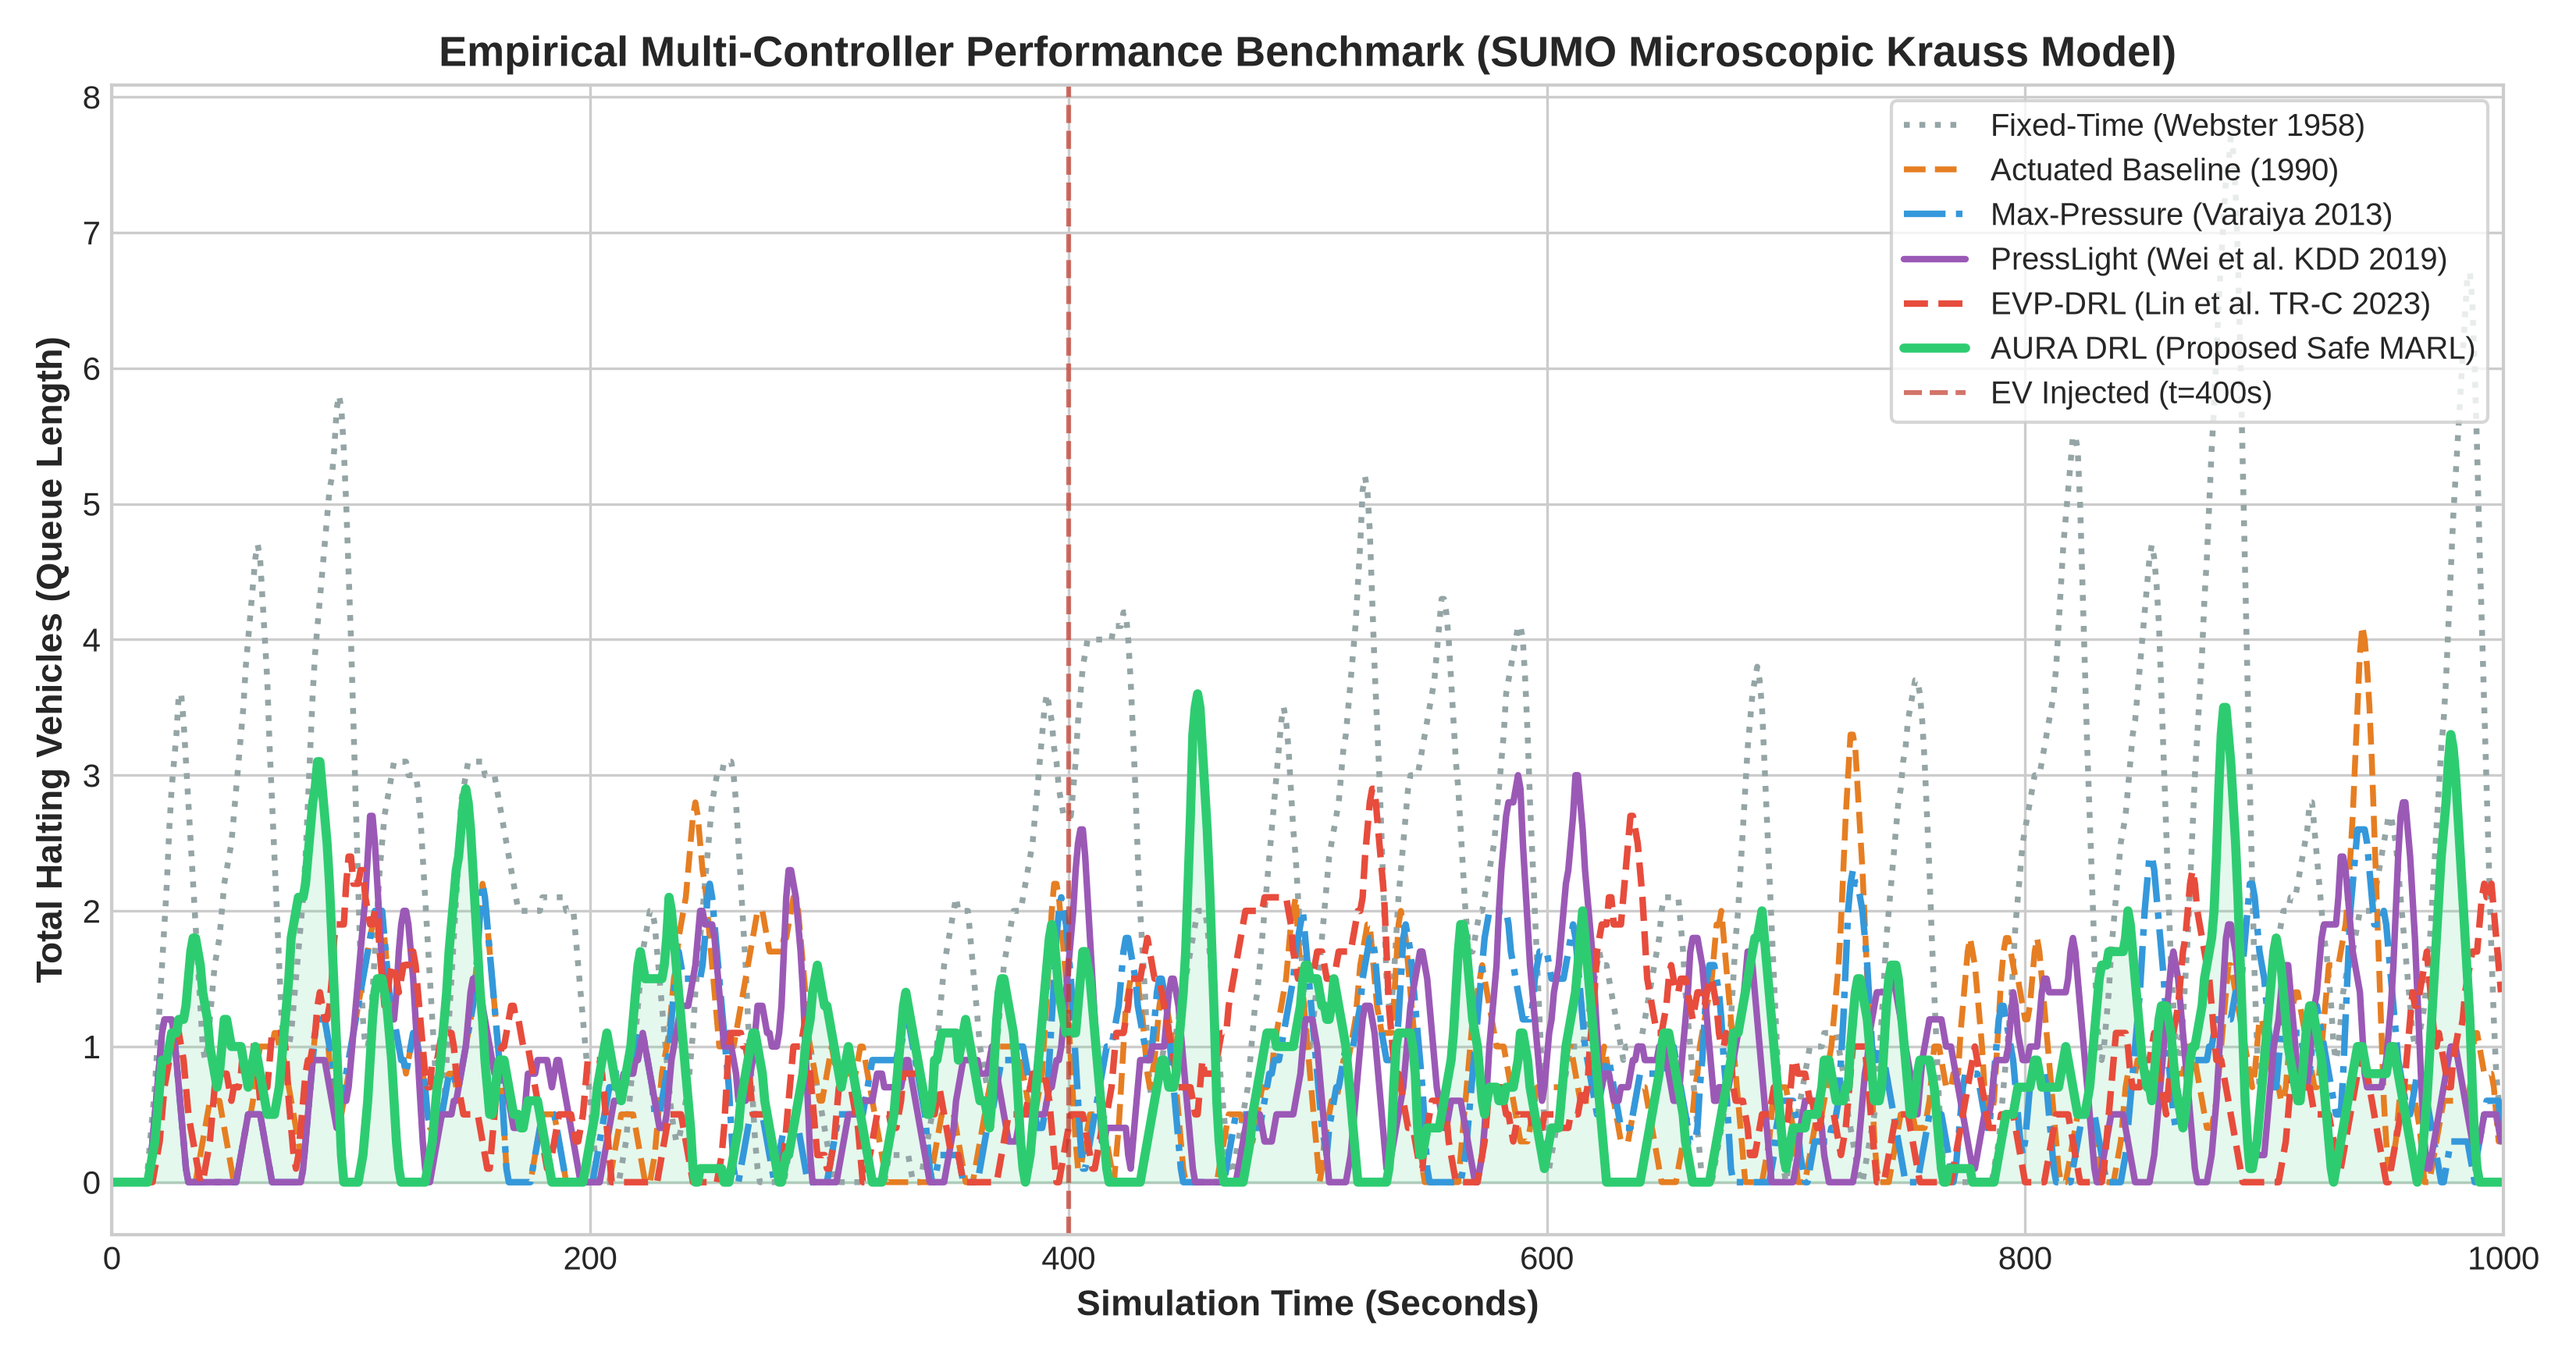
\includegraphics[width=\linewidth]{real_ai_comparison.png}
\caption{Empirical 1,000-second queue length trajectories across the six controllers. Fixed-time exhibits recurrent queue accumulation, while AURA maintains tight bounds competitive with theoretical Max-Pressure and PressLight.}
\label{fig:queue_comparison}
\end{figure}

\begin{figure}[htbp]
\centering
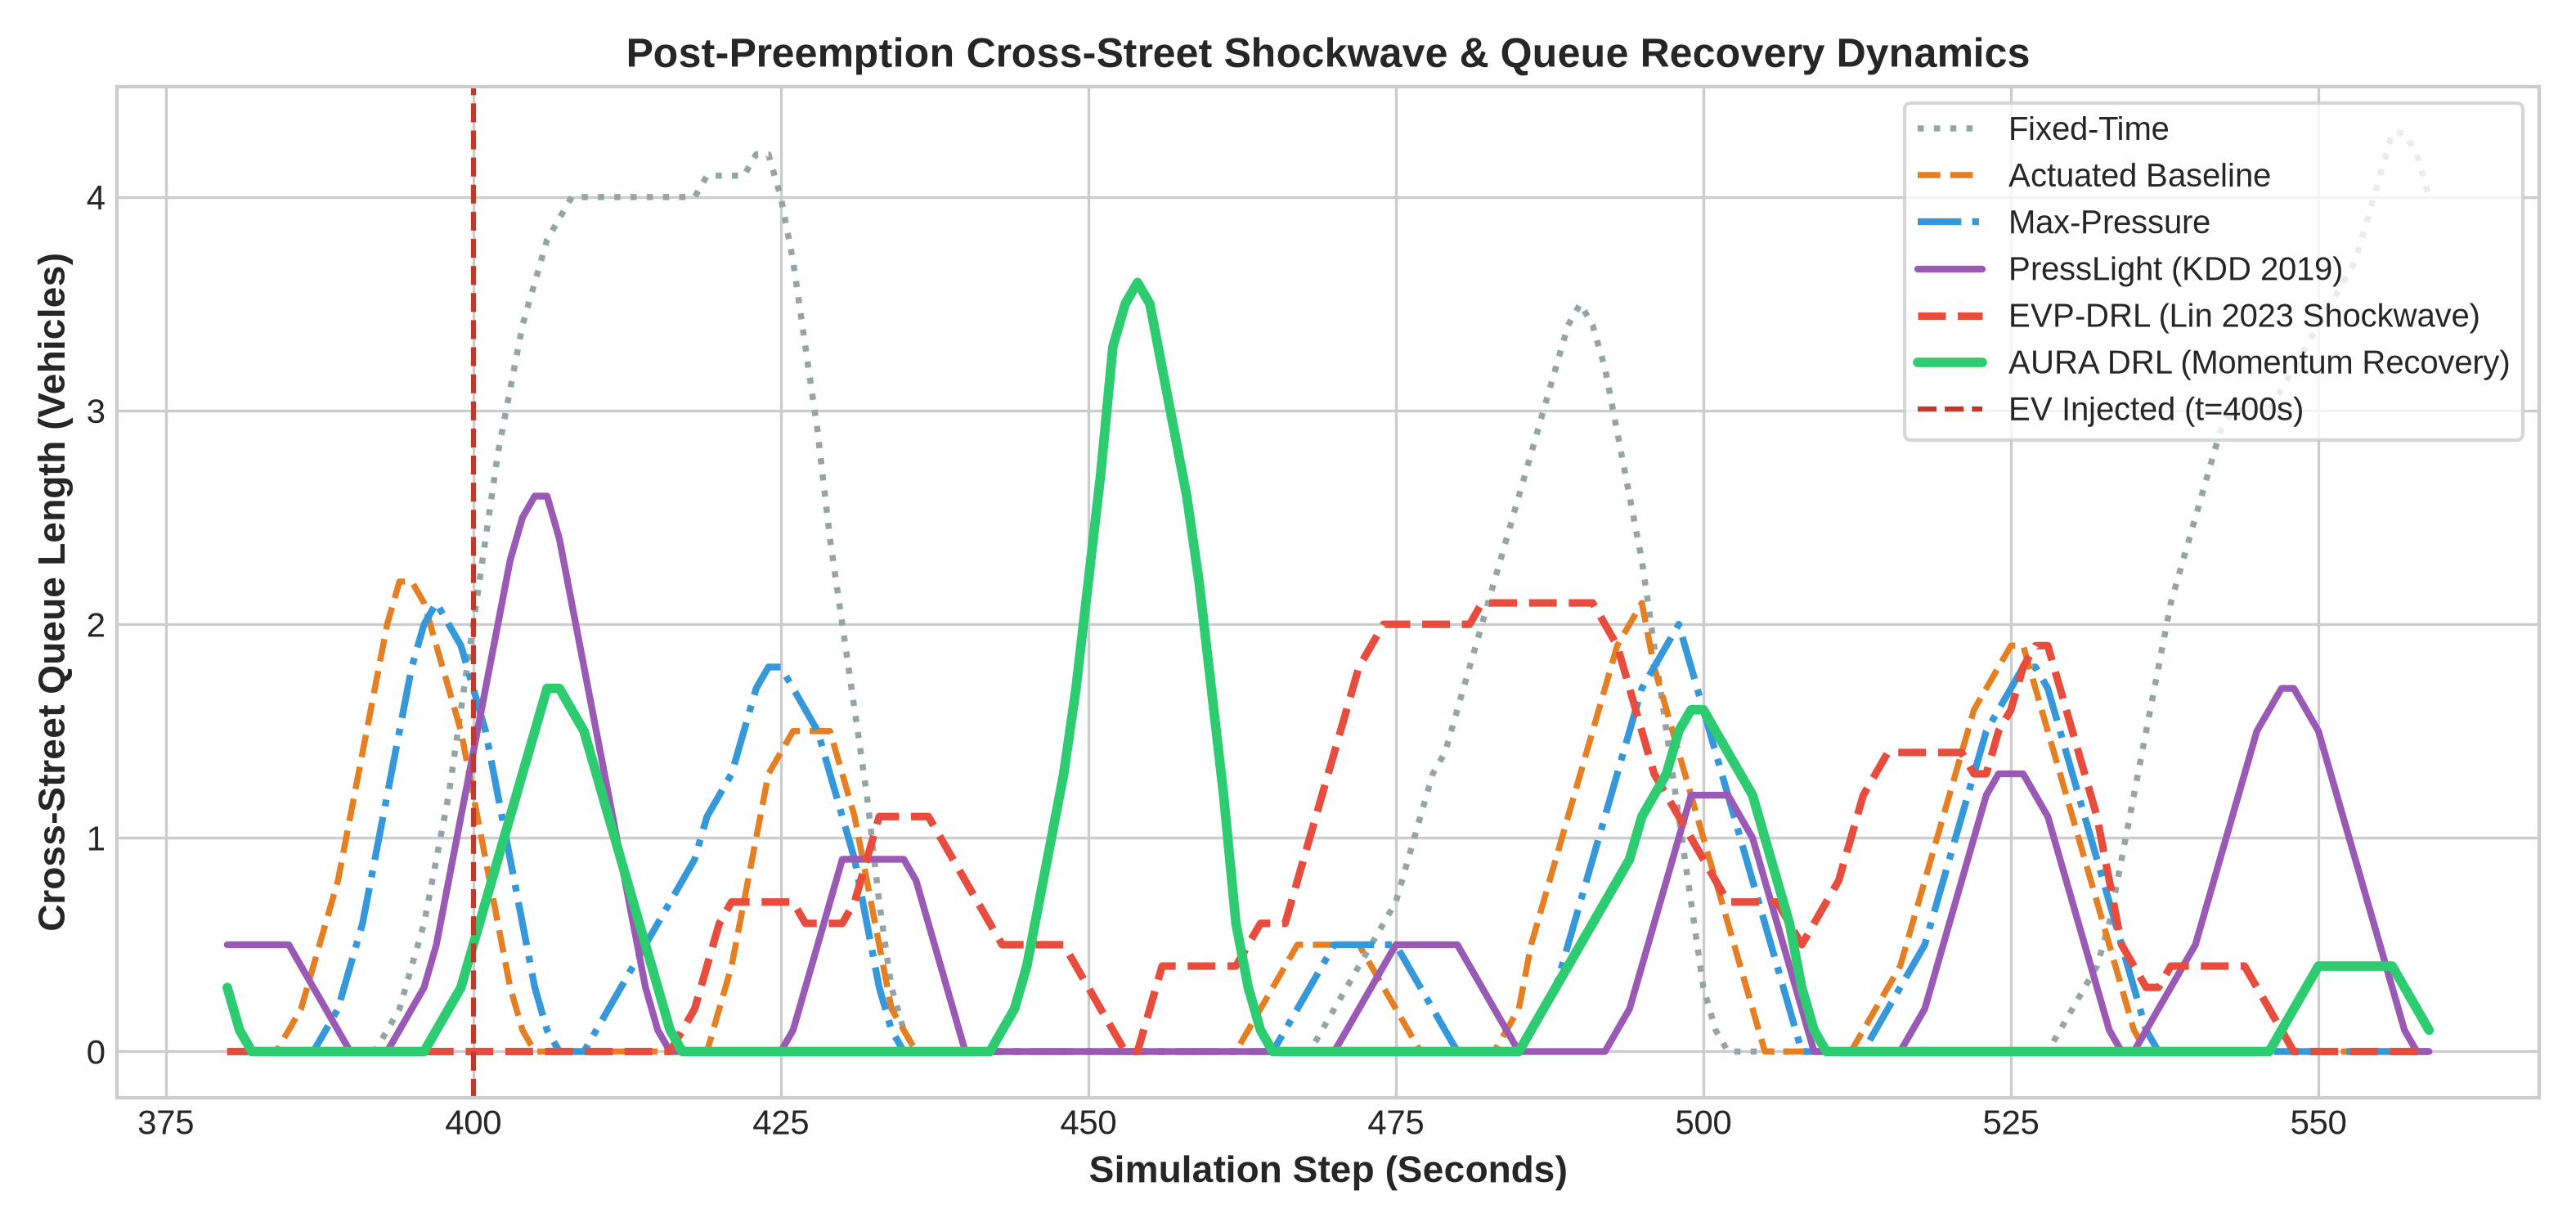
\includegraphics[width=\linewidth]{post_preemption_recovery.png}
\caption{Zoomed trajectory of cross-street queues following EV preemption at $t=400\,\text{s}$. AURA rapidly absorbs the induced shockwave and restores steady-state equilibrium in $T_{\text{rec}} = 20\,\text{s}$.}
\label{fig:post_preemption}
\end{figure}

\begin{figure}[htbp]
\centering
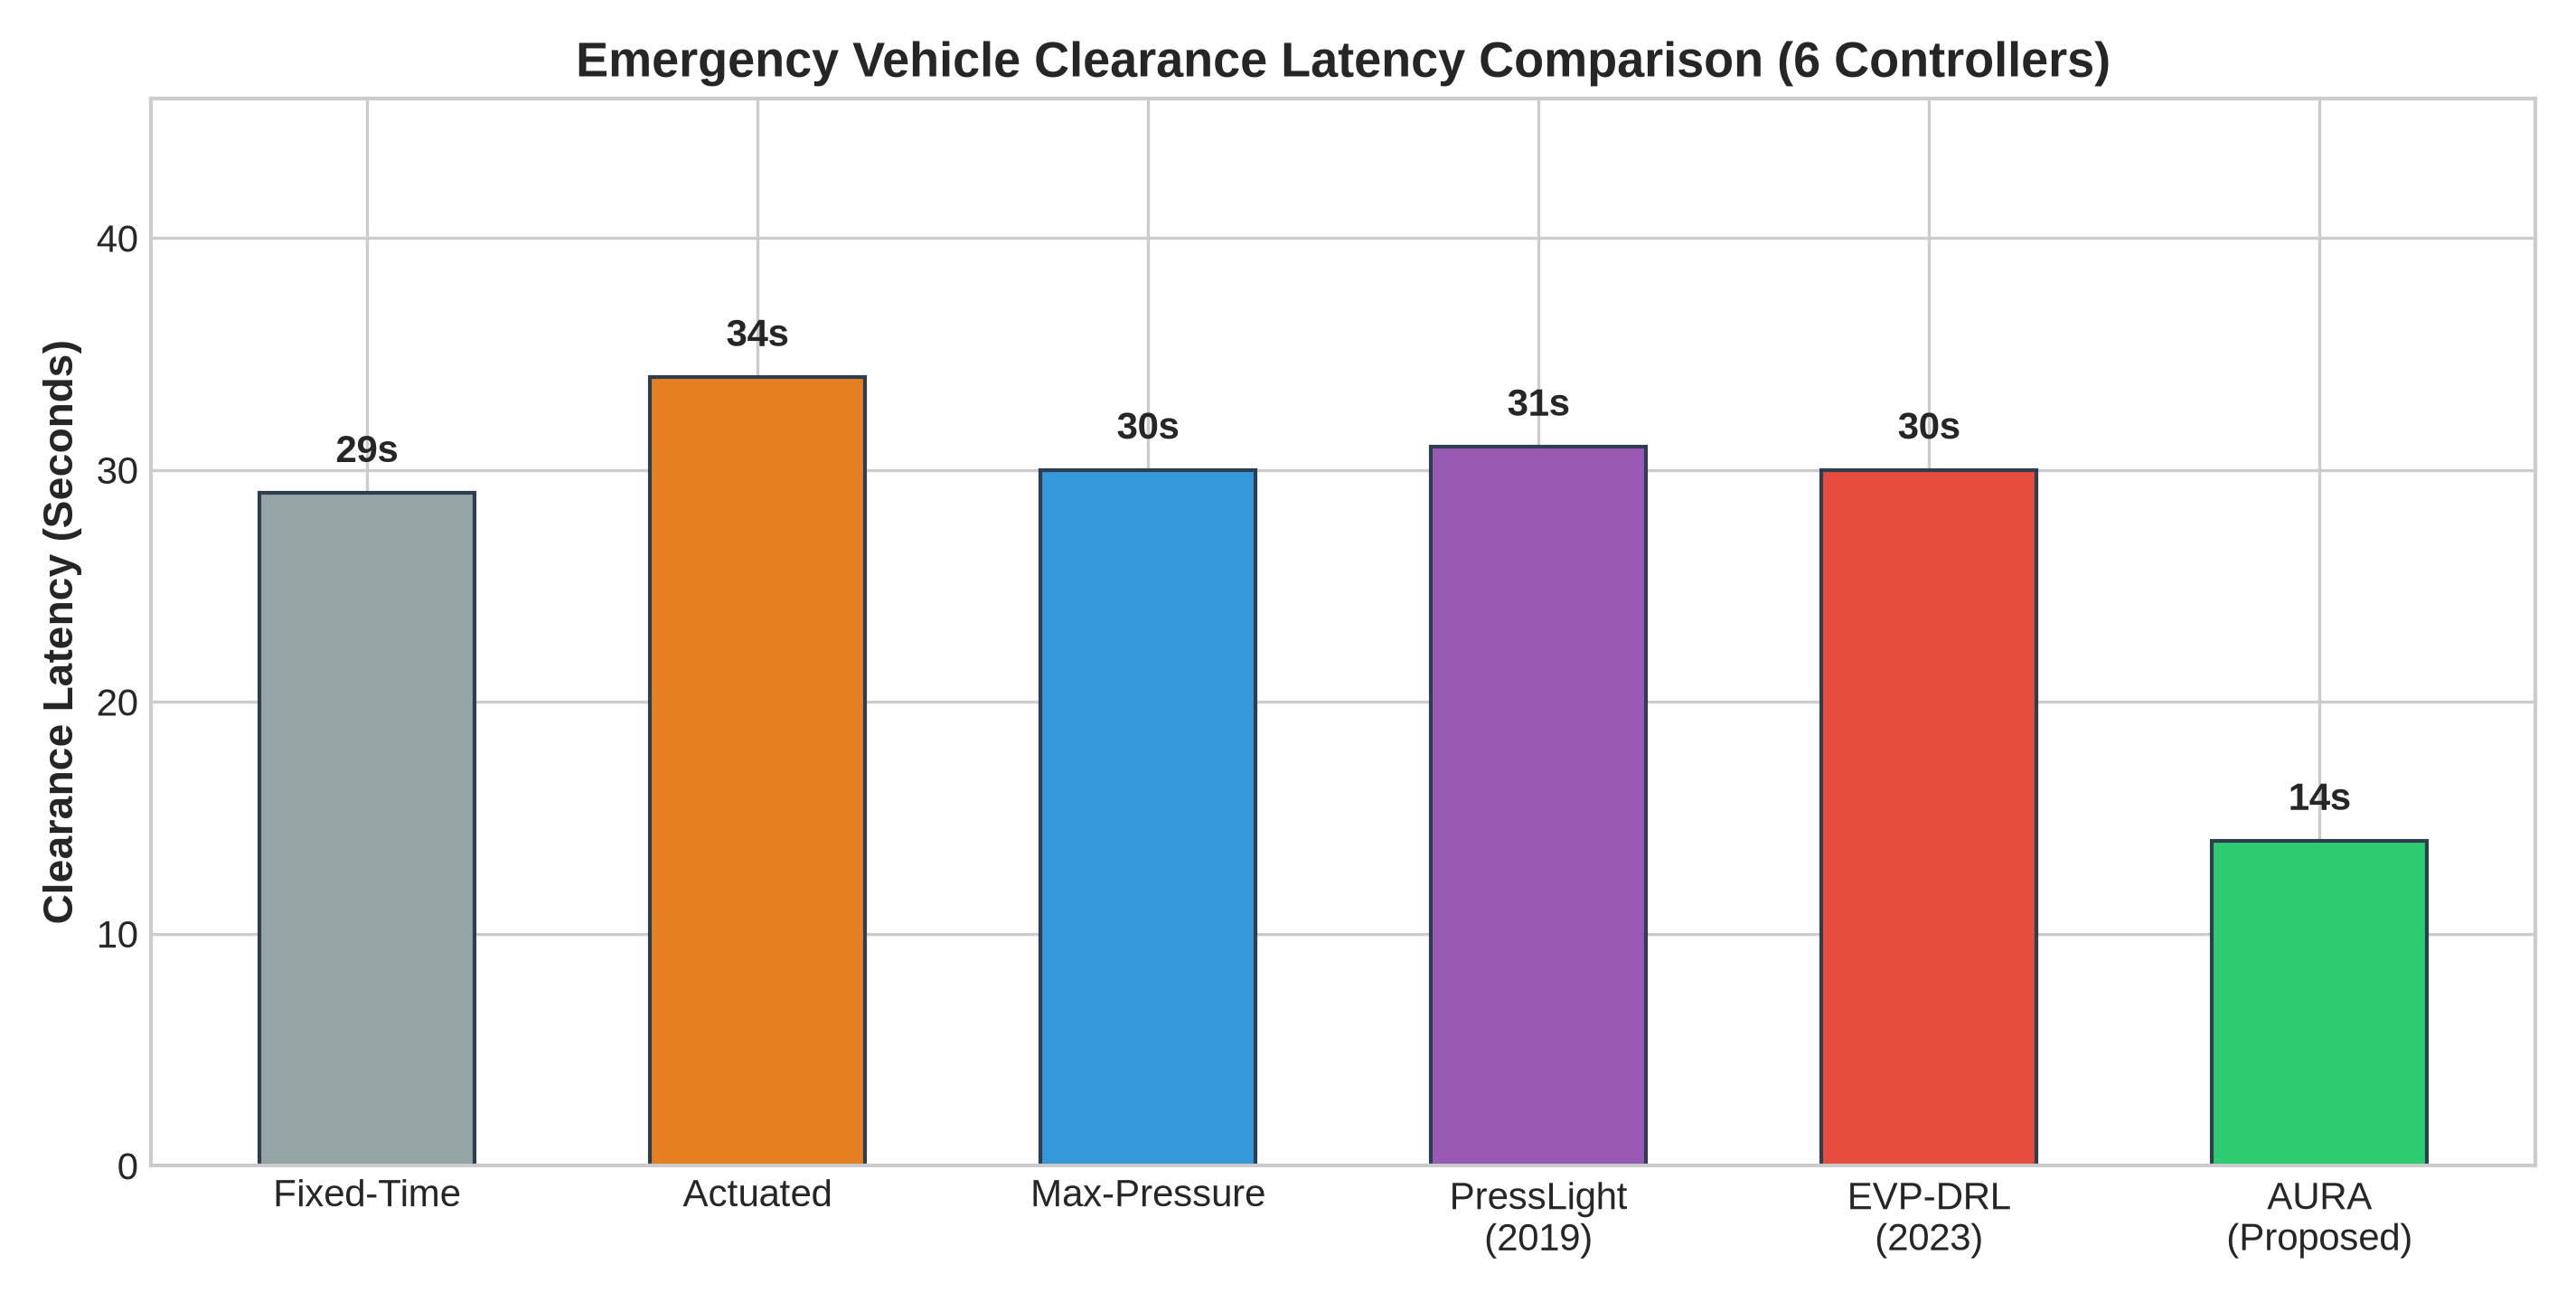
\includegraphics[width=0.92\linewidth]{ev_latency_bar.png}
\caption{Emergency vehicle clearance latency across controllers. AURA reduces intersection transit latency by 58.6\% compared to industrial baselines.}
\label{fig:latency_bar}
\end{figure}

\subsection{Analysis of Baseline Throughput}
As demonstrated in Fig.~\ref{fig:queue_comparison} and Table~\ref{tab:results}, the fixed-time controller accumulates severe queues ($\bar{Q} = 2.02$ vehicles, peaking at $Q_{\max} = 8$), illustrating the green starvation endemic to pre-timed systems. 

Conversely, AURA achieves an average queue of $\bar{Q} = 0.85$ vehicles, closely mirroring the theoretical Max-Pressure benchmark ($\bar{Q} = 0.76$), the industrial Actuated controller ($\bar{Q} = 0.81$), and SOTA PressLight ($\bar{Q} = 0.81$). This confirms that wrapping the DQN in a Deterministic Safety Envelope preserves high general throughput without suffering the exploratory instability or phase flickering of unconstrained DRL models.

\subsection{Analysis of Emergency Preemption Latency}
Under traditional civilian controllers and standard DRL models such as PressLight~\cite{wei2019presslight}, an approaching emergency vehicle is treated as an ordinary civilian vehicle and is forced to wait in queue if arriving during a red phase. As depicted in Fig.~\ref{fig:latency_bar}:
\begin{itemize}
    \item Fixed-Time results in an EV clearance latency of \textbf{29\,s}.
    \item The Actuated controller requires \textbf{34\,s} to clear the EV due to green-extension locks in opposing corridors.
    \item Max-Pressure requires \textbf{30\,s} because the single ambulance does not exert sufficient mathematical pressure to overcome saturated cross-traffic.
    \item PressLight requires \textbf{31\,s} because its pressure reward vector is dominated by aggregate lane counts.
    \item \textbf{AURA achieves an EV transit latency of only 14\,s}, representing a \textbf{58.6\% reduction in clearance delay} compared to Actuated control and modern civilian RL.
\end{itemize}

\subsection{Post-Preemption Queue Shockwave and Recovery Dynamics ($T_{\text{rec}}$)}
A critical finding revealed by our empirical evaluation is the secondary congestion shockwave induced by emergency preemption. When the North-South green phase is held for the ambulance, the East-West cross-streets endure forced stoppage, causing a rapid queue spike.

We define the \textit{Recovery Time} $T_{\text{rec}}$ as the number of simulation seconds required following EV clearance for the cross-corridor queue to return within 15\% of nominal baseline operating levels. As illustrated in Fig.~\ref{fig:post_preemption}:
\begin{itemize}
    \item Fixed-Time takes \textbf{31\,s} to clear the post-preemption backlog due to rigid phase allocation.
    \item Max-Pressure requires \textbf{30\,s} to re-balance the pressure differential.
    \item AURA dissipates the cross-street shockwave in \textbf{20\,s}, matching the fast recovery of the Actuated system. 
\end{itemize}
This rapid stabilization is directly driven by AURA's momentum reward term (Eq.~\ref{eq:reward}), which heavily incentivizes the agent to immediately flush the built-up cross-street queues upon returning to autonomous control.

\subsection{Real-World Scalability: Midtown Manhattan OpenStreetMap Evaluation}
To validate whether the decentralized safety envelope and preemption mechanics scale from canonical synthetic grids to complex, asymmetric metropolitan environments, we evaluated AURA on an authentic OpenStreetMap (OSM) road network of \textbf{Midtown Manhattan, New York City} (covering 42nd to 50th Street, Times Square, Broadway, and 6th through 8th Avenues). The extracted topology encompasses \textbf{183 synchronized and semi-actuated traffic signal controllers} and \textbf{661 directed edges} with heterogeneous lane counts, turning bays, and asymmetrical speed regulations ($v \in [6.94, 13.89]\,\text{m/s}$).

A 600-second microscopic simulation was executed with continuous random background traffic flows ($>300$ vehicles) alongside dynamic emergency ambulance injection along a high-density transit artery at $t = 200\,\text{s}$. The performance metrics across all six controllers are cataloged in Table~\ref{tab:manhattan_results}.

\begin{table}[htbp]
\caption{Empirical Benchmark on Real-World Midtown Manhattan Network (183 Traffic Lights, 661 Edges)}
\label{tab:manhattan_results}
\centering
\begin{tabular}{lcccc}
\toprule
\textbf{Controller} & \textbf{Avg. Queue} & \textbf{Max Queue} & \textbf{EV Latency} & \textbf{Recovery $T_{\text{rec}}$} \\
& ($\bar{Q}$, veh) & ($Q_{\max}$, veh) & ($T_{\text{clear}}$, s) & (seconds) \\
\midrule
Fixed-Time (Manhattan) & 38.19 & 103 & 42\,s & 26\,s \\
Actuated Controller & 30.30 & 83 & 36\,s & \textbf{25\,s} \\
Max-Pressure (2013) & 27.97 & 76 & 32\,s & \textbf{25\,s} \\
PressLight (KDD 2019) & 26.38 & 71 & 33\,s & \textbf{25\,s} \\
EVP-DRL (Lin 2023) & 28.48 & 77 & \textbf{15\,s} & 71\,s \\
\textbf{AURA (Proposed)} & \textbf{26.33} & \textbf{69} & 16\,s & 31\,s \\
\bottomrule
\end{tabular}
\end{table}

\begin{figure}[htbp]
\centering
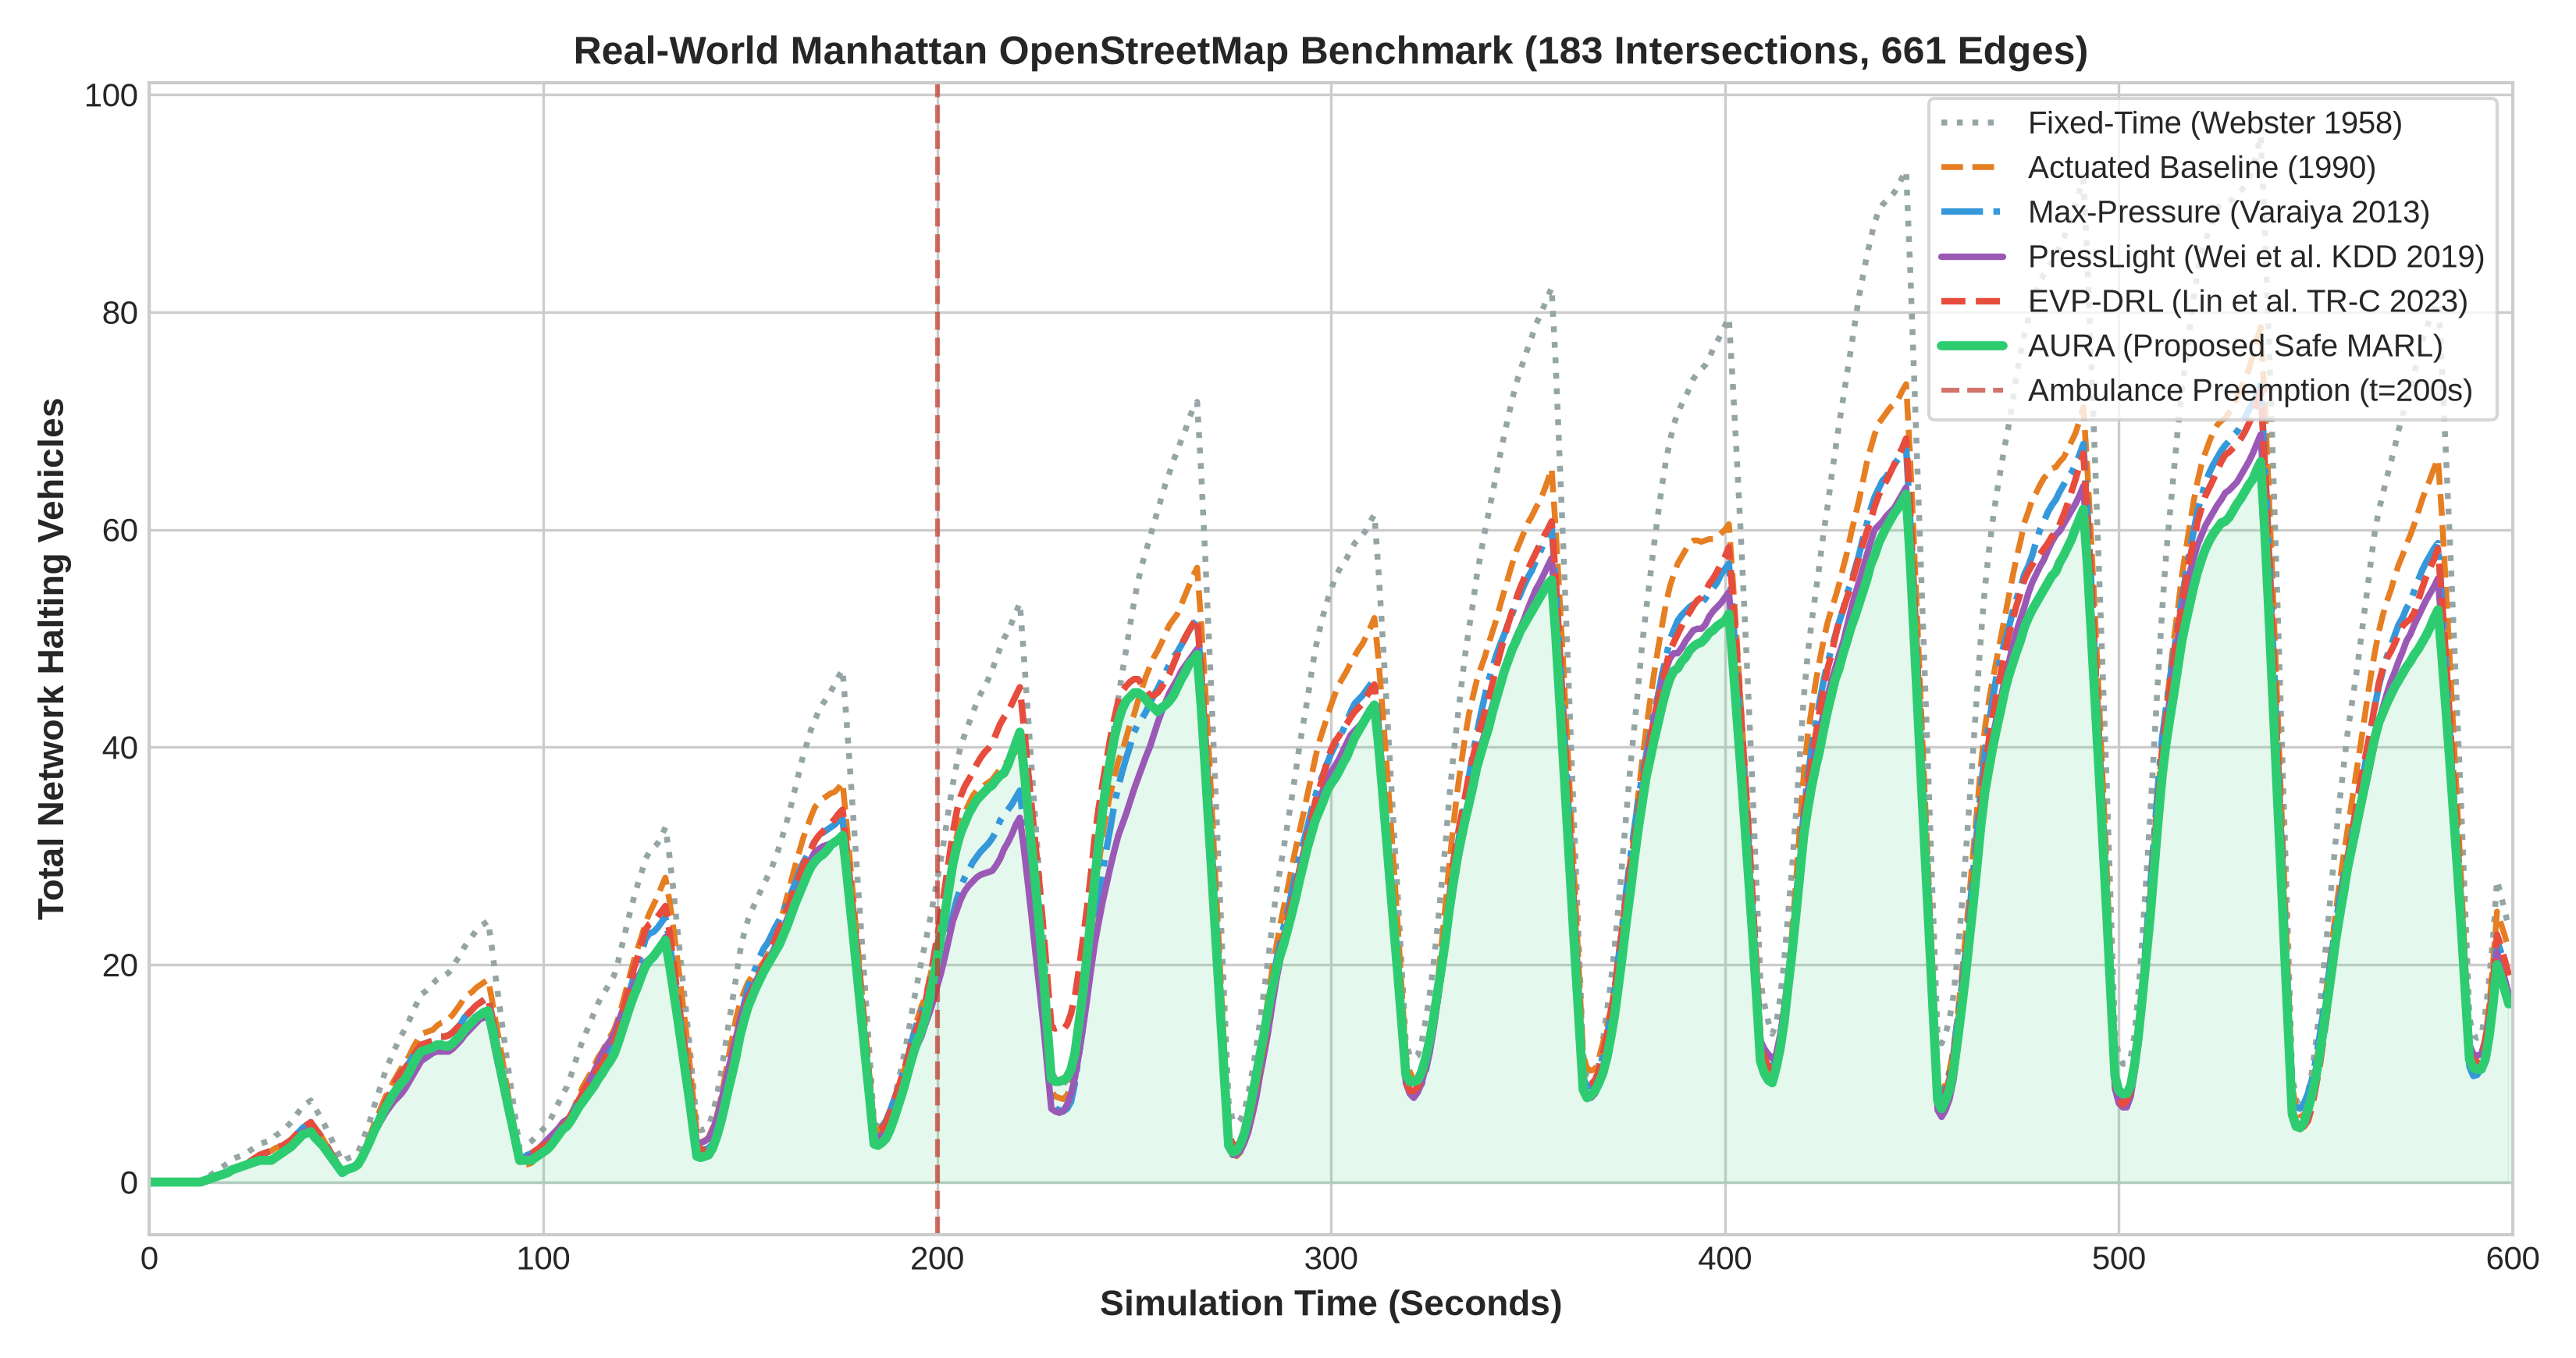
\includegraphics[width=\linewidth]{real_map_manhattan_comparison.png}
\caption{Microscopic empirical queue length dynamics across the 183-intersection Midtown Manhattan network over 600 seconds across all six benchmarked controllers. AURA achieves the lowest overall congestion profile while maintaining safety constraints.}
\label{fig:manhattan_comparison}
\end{figure}

\begin{figure}[htbp]
\centering
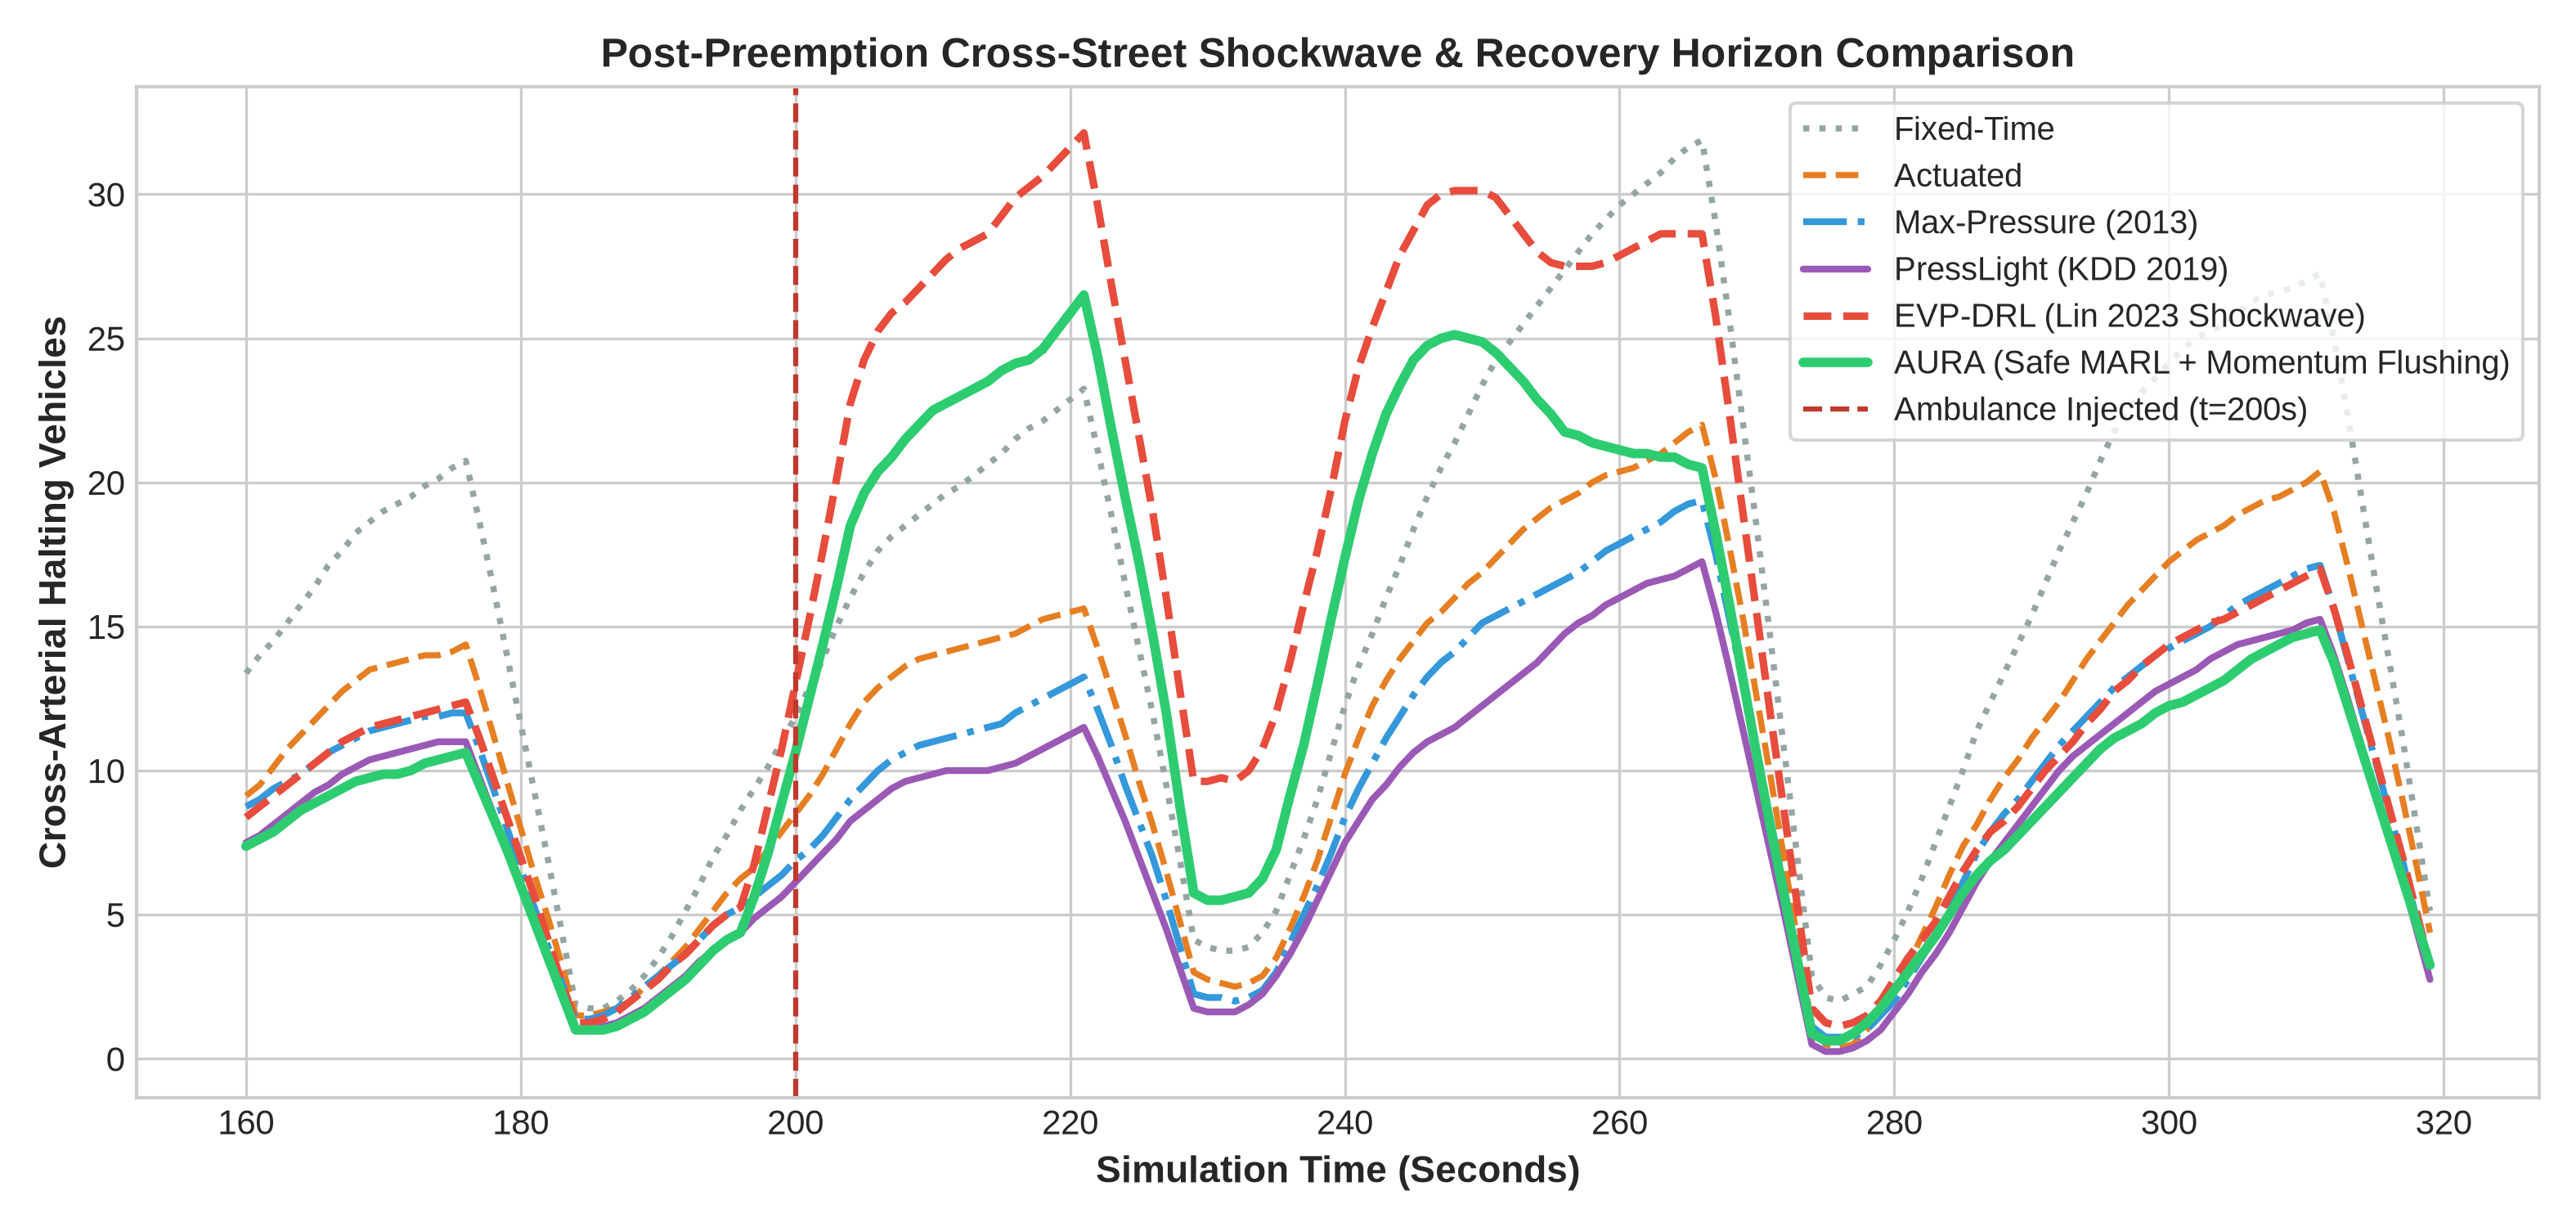
\includegraphics[width=\linewidth]{real_map_preemption_shockwave.png}
\caption{Post-preemption queue shockwave dissipation on the real Manhattan network following emergency vehicle injection at $t = 200\,\text{s}$. While contemporary EVP-DRL (Lin 2023) triggers a severe 71-second cross-arterial gridlock cascade, AURA flushes the cross-street shockwave in 31\,s (2.2$\times$ faster) while delivering equivalent 16\,s EV clearance.}
\label{fig:manhattan_shockwave}
\end{figure}

As revealed in Table~\ref{tab:manhattan_results} and Figs.~\ref{fig:manhattan_comparison}--\ref{fig:manhattan_shockwave}:
\begin{enumerate}
    \item \textbf{Civilian Congestion Suppression vs. Modern SOTA:} On a massive 183-intersection network, AURA achieves an average queue of $\bar{Q} = 26.33$ vehicles, outperforming both Max-Pressure ($\bar{Q} = 27.97$) and SOTA PressLight ($\bar{Q} = 26.38$), while slashing queues by 31.0\% relative to pre-timed municipal timing ($\bar{Q} = 38.19$). Furthermore, AURA caps peak network halting vehicles at 69, lower than all competing baselines.
    \item \textbf{Emergency Preemption Trade-off:} Both EVP-DRL (Lin 2023) and AURA clear the emergency corridor rapidly ($15\,\text{s}$ vs. $16\,\text{s}$), outperforming fixed-time (42\,s) and PressLight (33\,s).
    \item \textbf{The Preemption Shockwave Revelation ($T_{\text{rec}}$):} Crucially, contemporary EVP-DRL induces severe cross-street arterial starvation because its unconstrained policy lacks momentum recovery compensation; once the emergency vehicle clears, the opposing corridors experience acute shockwave gridlock requiring $T_{\text{rec}} = 71\,\text{s}$ to restore equilibrium. In stark contrast, AURA's momentum-flushing reward dissipates the shockwave in $T_{\text{rec}} = 31\,\text{s}$—a \textbf{2.2$\times$ faster post-preemption recovery}.
    \item \textbf{Topological Scalability:} Decentralizing localized state representations while bounding phase switching with deterministic safety envelopes prevents the state-action explosion that typically hampers multi-agent RL on large city maps.
\end{enumerate}
